
In this section we will look at what can be done when the process dynamics
are unknown.
In this case we cannot calculate directly neither $r$, $T_\pi Q$ nor
$TQ$ because the transition and reward kernels $P,R$ are unknown.

It is clear that \cref{alg:theoSimpleQ} will not work without
modification in this case. Simply because $R$ and $P$ are not
available.
To make the scheme work anyway we could simply avoid taking expectations
and use the random outcomes of the kernels.
Leading to

\begin{figure}[H]
\begin{algorithm}[H] %\label{algocf:fq} % this labels line, could not fix
  \caption{Random theoretical Q-iteration (example of thought)}
\KwIn{MDP $(\cl{S}, \cl{A}, P, R, \gamma)$, number of iterations $K$}
$\forall (s, a) \in \cl{S} \times \cl{A} :
\wt{Q}_0(s, a) \leftarrow X \sim R(\cdot \mid s, a)$.

\For{$k = 0,1,2,\dots,K-1$}{
  $ \forall (s, a) \in \cl{S} \times \cl{A} :
  \wt{Q}_{k+1}(s, a) \leftarrow r'
  + \gamma \sup_{a' \in \cl{A}} \wt{Q}_k(s', a')$

  where $r' \sim R(\cdot \mid s, a), s' \sim P(\cdot \mid s, a)$.
}
Define $\pi_K$ as the greedy policy w.r.t. $\wt{Q}_K$ \\
\KwOut{An estimator $\widetilde{Q}_K$ of $Q^*$ and policy $\pi_K$}
\label{alg:theoRandomQ}
\end{algorithm}
\end{figure}
We immedially run into problems in the uncountable case, because
drawing uncountably many times from a distribution is not easily
defined in a sensible way.
Even in the finite case where the functions $\wt{Q}_k$
are well defined, they cannot converge if $R$ is not deterministic.
Therefore this approach does not work in a continuous or
stochastic setting.

There are broadly two ways of dealing with these problems.
In the \emph{indirect} approaches one tries to first estimate $P$ and $R$
by sampling.
Then since $P$ and $R$ are now ``known'' we can apply the model-dependent
methods.
The \emph{direct} approaches broadly cover \emph{the rest} of the 
cases, and it is mainly these were are going to look at throughout this
paper. A popular indirect approach is called
\emph{temporal difference} (TD) learning 

\section{Finite case}

TD learning is based on the following
update scheme
\begin{equation}
  \wt{Q}_{k+1}(s, a) \leftarrow (1-\alpha_k) \wt{Q}_k(s, a)
  + \alpha_k (r' + \gamma \cdot \max_{a' \in \cl{A}} \wt{Q}_k(s', a'))
  \label{eq:tdeq}
\end{equation}
Here $r'$ and $s'$ are the reward and next-state drawn from the
reward and transition kernels,
and $\alpha_k \in [0,1]$ is the so-called \defemph{learning rate}
(of the $k$th step).
The 'temporal difference' is also the name of term
$ \alpha_k ( r' + \gamma \cdot \max_{a \in \cl{A}} \wt{Q}_k(s', a')
- \wt{Q}_k(s, a) )$ occuring from rearranging \cref{eq:tdeq}.
Usually the learning rate is fixed before running the algoritm
(does not depend on the history) and is set to decay
from 1 to 0 in some fashion as $k \to \infty$.

We will now look at a convergence result originally obtained in
\mcite{WD92} of a TD algorithm using Q-functions.
The result was extended slightly in \mcite{J94} and is here presented
more in the style of \ncite{J94}.
\begin{figure}[H]
\begin{algorithm}[H] %\label{algocf:fq} % this labels line, could not fix
  \caption{Finite asynchronos Q-learning}
  \KwIn{MDP $(\cl{S}, \cl{A}, P, R, \gamma)$ such that
    $\abs{\cl{S}}\abs{\cl{A}} < \infty$,
    number of iterations $K$,
    state-action pairs $(s_1,a_1, \dots, s_K, a_K)$,
    learning rates $(\alpha_1', \dots, \alpha_K')$,
    initial $\wt{Q}_0 : \cl{S}\times\cl{A} \to \R$
  }
  Put $\alpha_k(s, a) \leftarrow \begin{cases}
    \alpha'_k & (s, a) = (s_k, a_k)
    \\ 0 & (s, a) \neq (s_k, a_k)
  \end{cases}$.

  \For{$k = 1,2,\dots,K$}{
    Sample $r' \sim R(\cdot \mid s_k, a_k),
    s' \sim P(\cdot \mid s_k, a_k)$

    Update action-value function:
    \[ \wt{Q}_k \leftarrow
      \wt{Q}_{k-1} +
      \alpha_k (r' + \max_{a' \in \cl{A}} \wt{Q}_{k-1}(s', a'))
    \]
  }
  Define $\pi_K$ as the greedy policy w.r.t. $\wt{Q}_K$ \\
  \KwOut{An estimator $\widetilde{Q}_K$ of $Q^*$ and policy $\pi_K$}
  \label{alg:finAsyncQL}
\end{algorithm}
\end{figure}
Note that only the value of the pair $(s_k, a_k)$ are updated in each
step of the algorithm
(since $\alpha_k(s, a) = 0$ for all $(s,a)\neq(s_k, a_k)$).

\begin{thm}[Watkins, Dayan 1992]
  Let $s_1, a_1, s_2, a_2, \dots \in
  \cl{S} \times \cl{A} \times \cl{S} \times \cl{A} \times \dots$
  be random variables, and $\alpha_1, \alpha_2, \dots \in [0,1]$.
  The output $\wt{Q}_K$ of \cref{alg:finAsyncQL} converges to $Q^*$
  provided
  \begin{enumerate}
    \item $\Prob\left(\sum_{i=1}^\infty \alpha_i(s,a) = \infty\right) = 1,
      \Prob\left(\sum_{i=1}^\infty \alpha_i^2(s,a) < \infty\right) = 1$.
    \item $\Var(R(\cdot \mid s, a)) < \infty$ for all $(s, a) \in
      \cl{S}\times\cl{A}$.
    \item If $\gamma = 1$ all policies lead to a reward-free terminal
      state almost surely.
  \end{enumerate}
\end{thm}
In the original formulation the sums of learning rates were supposed to
converge \emph{uniformly}. However this is equivalent to this formulation
because of the fact that
$\Prob(\sup_{(s, a) \in \cl{S} \times \cl{A}} \abs{f_n(s, a)} \to 0) = 1 \iff
\Prob\left(\;\abs{f_n(s, a)} \to 0 \right) = 1,
\forall (s, a) \in \cl{S} \times \cl{A}$
whenever $\cl{S}, \cl{A}$ is finite.
Notice that the first condition implies that all state-action pairs
occur infinitely often almost surely.
Also notice that the second condition is automatically fulfilled under
(D) since then $\Var(R(\cdot \mid s, a)) \leq \E (2R_{\max})^2 = 4 R_{\max}^2$.

%% Szepesvári Asymptotic convergence-rate of Q-learning 1997
In a special case of the same setup, convergence rates where
established by \mcite{S97}.
\begin{thm}[Szepesvári]
  Let $t \in \N$ and
  $s_1, a_1, s_2, \dots, s_t, a_t$ be sampled i.i.d. from
  $p \in \cl{P}(\cl{S} \times \cl{A})$.
  Set the learning rates such that
  $\alpha'_k
  = |\{ i \in [k-1] \mid (s_i, a_i) = (s_k, a_k) \}|^{-1}$,
  i.e. the reciprocal of the frequency of $(s_k, a_k)$ at step $k$.
  Let $\beta = \max_{x \in \cl{S} \times \cl{A}} p(x) /
  \min_{x \in \cl{S} \times \cl{A}} p(x)$.
  Then for some $B > 0$ the following holds asymptotically almost surely
  \begin{equation}
    \abs{\wt{Q}_t - Q^*} \leq B \frac{1}{t^{\beta (1-\gamma)}}
    \label{eq:Szepesvari1}
  \end{equation}
  and
  \begin{equation}
    \abs{\wt{Q}_t - Q^*} \leq B \sqrt{\frac{\log \log t}{t}}
    \label{eq:Szepesvari2}
  \end{equation}
\end{thm}
Here \cref{eq:Szepesvari1} is tightest when $\gamma > 1 - \beta/2$
otherwise \cref{eq:Szepesvari2} is tighter.
%todo find out if we wanna do proof

A paper \mcite{MH18} proves that $Q$-learning is PAC-learnable
given some additional assumptions.

\begin{algorithm}[H] %\label{algocf:fq} % this labels line, could not fix
  \caption{Finite synchronos Q-learning}
  \KwIn{MDP $(\cl{S}, \cl{A}, P, R, \gamma)$ such that
    $\abs{\cl{S}}\abs{\cl{A}} < \infty$,
    number of iterations $K$,
    learning rates $(\alpha_1, \dots, \alpha_K)$,
    initial $\wt{Q}_0 : \cl{S}\times\cl{A} \to \R$
  }

  \For{$k = 1,2,\dots,K$}{
    Sample $r' \sim R(\cdot \mid s_k, a_k),
    s' \sim P(\cdot \mid s_k, a_k)$

    Update action-value function:
    \[ \wt{Q}_k \leftarrow
      \wt{Q}_{k-1} +
      \alpha_k (r' + \max_{a' \in \cl{A}} \wt{Q}_{k-1}(s', a'))
    \]
  }
  Define $\pi_K$ as the greedy policy w.r.t. $\wt{Q}_K$ \\
  \KwOut{An estimator $\widetilde{Q}_K$ of $Q^*$ and policy $\pi_K$}
  \label{alg:finSyncQL}
\end{algorithm}


\begin{thm}[Mansour 2003]
  Assume (P) and (D). Let $\alpha_k = 1/(k+1)^\omega$ where
  $\omega \in (1/2,1]$.
  Fix $C>0$, a sufficiently large constant.
  Let $\ve, \delta >0$ and define
  \[ A = \frac{4V^2_{\max} \log(2\abs{\cl{S}}\abs{\cl{A}} V_{\max}/\delta
  (1-\gamma)\ve)}{(1-\gamma)^2\ve^2}, \quad B= 2 \log(V_{\max}/\ve)/(1-\gamma) \]
  The following hold for any $\psi > 0$.

  If the synchronos algorithm (\cref{alg:finSyncQL}) is run with
  \[ K \geq C \begin{cases}
      A^{1/\omega} + B^{1/(1-\omega)} & \omega \in (1/2,1)
      \\ \frac{(2 + \psi)^B}{\psi^2} \left(A +
      \frac{4 V^2_{\max} \log(1/\psi)}{(1-\gamma)^2 \ve^2} \right)
      & \omega = 1
    \end{cases}
  \]
  then with probability at least $1-\delta$ we have
  $\norm{\wt{Q}_K - Q^*}_\infty < \ve$.

  If the asynchronos algorithm (\cref{alg:finAsyncQL}) with 
  \[ K \geq C \begin{cases}
      (L^{1 + 3 \omega} A)^{1/\omega} + (L B)^{1/(1-\omega)}
      & \omega \in (1/2,1)
      \\ \frac{(L + \psi L + 1)^B}{\psi^2}
      \left(A + \frac{4V^2_{\max} \log(1/\psi)}{(1-\gamma)^2\ve^2} \right)
	& \omega = 1
  \end{cases} \]
  and the state-action pairs $(s_1, a_1, \dots, s_K, a_K)$ are drawn
  from a distribution such that every pair in $\cl{S}\times\cl{A}$
  appears in every sequence of length at least $L > 0$,
  then with probability at least $1-\delta$ we have
  $\norm{\wt{Q}_K - Q^*}_\infty < \ve$.
  \label{thm:mansour2003}
\end{thm}
In \ncite{MH18} $L$ is called the \emph{covering rate}.

\begin{rem}
An interesting side note to \cref{thm:mansour2003} is that
one can use the bounds to give hints at how to tune the learning rate
by changing $\omega$. Optimizing for different scenarios yield
different learning theoretically optimal values for $\omega$.
For example if we want to optimize for the bound on $K$ for 
$\gamma \to 1$ using the synchronos algorithm,
we get the following rate (treating other variables as constant)
$K \geq C'(1/(1-\gamma)^{4/\omega} + 1/(1-\gamma)^{1/(1-\omega)})$
for some $C'>0$.
Thus picking $\omega = 4/5$ is optimal.
As another example: running the asynchronos algorithm and wanting to
minimize for large covering rates $L$. We get
$K \geq C''(L^{2+1/\omega} + L^{1/(1-\omega)})$
for some $C'' > 0$.
This is optimized for $\omega \approx 0.77$.
Then in \ncite{MH18} experiments points to $\omega = 0.85$ as being
optimal using a scheme generating random finite MDPs.
Other authors have since used this number as a standard
value for the learning rate
(see e.g. \mcite{DM17}) % todo find more examples
\end{rem}

\subsection{History dependent setting}

\begin{sett}[Finite HDP]
  \leavevmode
  \begin{enumerate}
    \item A history dependent decision process (see \cref{sett:HDP}),
      with a single \emph{finite} state space,
      a single finite action space $(\cl{S}, \cl{A})$,
      and transition and reward kernels $(P_n, R_n)_{n \in \N}$.
      Define $\cl{H}^* \defeq \bigcup_{i \in \N} \cl{H}_n$,
      the space of finite histories.
    \item $(P_n)_{n \in \N}$ is viewed as a single kernel
      $P : \cl{H}^* \times \cl{A} \leadsto \cl{S}$.
    \item $(R_n)_{n \in \N}$ is deterministic and viewed as a single function
      $r : \cl{H}^* \to \R$.
      This is discounted by $\gamma \in [0,1)$ in accordance to
      condition (D). That is
      $r(h_n)$ is bounded in the interval
      $[-\gamma^{n-2}R_{\max}, \gamma^{n-2} R_{\max}]$ for any
      $h_n \in \cl{H}_n$.
      Furthermore $r$ depends only on $s_1 a_1 \dots s_k r_{k-1} a_k$
      when evaluated on
      $h_{k+1} = s_1 a_1 \dots r_{k-1} a_k s_{k+1} \in \cl{H}_{k+1}$.
  \end{enumerate}
  \label{sett:HDP_MH}
\end{sett}

\begin{rem}
  Note that the finite \cref{sett:HDP_MH} is a special case of
  \cref{sett:Schal} considered by [Schäl, 1974],
  because Polishness and compactness of $\cl{S}, \cl{A}$ is readily
  implied by using the discrete topology in the finite state and action
  spaces, and the fact that (D) implies pt. 5 in \cref{sett:Schal}.
  Further the conditions (S) and (W) of Schal are also both implied by
  the discreteness.
  This implies by \cref{thm:SchalExi} the existence of an optimal
  $\pi^* \in R\Pi$ and that $V^*_n \to V^*$.
\end{rem}

Within \cref{sett:HDP_MH} Q-functions are generalized so that
they are taking values in $\cl{H}^* \times \cl{A}$.
We likewise generalize the $T$ function by
\begin{equation}
  TQ(h, a) \defeq r' +
  \gamma \sum_{s\in\cl{S}} \max_{a' \in \cl{A}} Q(hr'as, a') P(s \mid ha),
  \qquad r' = r(h, a)
  \label{eq:MH_Q_def}
\end{equation}

The optimal Q-function $Q^*$ is defined in [Majeed, Hutter] as
the fixed point of the $T$ operator in
$\cl{L}_\infty(\cl{H}^* \times \cl{A})$.
%todo prove that this is the normal sup definition

Now a function $\phi : \cl{H}^* \to \cl{X}$ is introduced
which maps a history to a new finite space $\cl{X}$.
The intuition here is that $x_n = \phi(h_{n-1} r_{n-2} a_{n-1} s_n)$ is the
state $s_n$ as it is perceived by the agent.
This is called \defemph{partial observability}.
$\phi$ is a assumed to be surjective so $\cl{X}$ is a finite space of
reduced size in comparison to $\cl{S}$.
In applications this could be a partially observable environment
or a latent space.

This way we are now considering a class of problems
which is wider than a 
history dependent decision process (HDP).
Namely a partially observable HDP or shortened: POHDP.
A HDP under \cref{sett:HDP_MH} is the subclass of POHDP where
$\cl{S} = \cl{X}$ and $\phi = \id_\cl{S}$.

Let $\phi_{hra}(s) = \phi(hras)$. Then we can define a kernel
\begin{align*} p_h & : \{\phi(h)\} \times \cl{A} \leadsto \cl{X}
  \\ p_h & (x' \mid xa)
  = \sum_{s:\phi(hr'as)=x'} P(s \mid ha), \quad r'=r(h,a)
\end{align*}
or expressed as an image measure
$p_h(\cdot \mid xa) = \phi_{hr'a}(P(\cdot \mid ha))$.
and further function $q_h^*$ by the equation
\begin{equation}
  q_h^*(x, a) = r' + \gamma \sum_{x' \in \cl{X}} 
  \max_{a' \in \cl{A}} q^*_h(x', a')
  p_h(x' \mid xa), \quad r'=r(h,a)
  \label{eq:MH_q_def}
\end{equation}

\begin{asm}[State-uniformity condition]
  For any $h,h' \in \cl{H}^*$ we have
  \[ \phi(h) = \phi(h') \implies Q^*(h, \cdot) = Q^*(h', \cdot) \]
  \label{asm:stateUniformity}
\end{asm}

A process as in \cref{sett:HDP_MH} together with the state-uniformity condition
is by \ncite{MH18} called a \emph{Q-Value uniform decision process} (QDP).

\begin{thm}[Hutter, 2016]
  Under \cref{asm:stateUniformity} we have
  $q^*_{h'}(\phi(h), a) = Q^*(h, a)$ for any $h'\in \cl{H}^*$.
\end{thm}

With this as a motivation we will try to use
the standard TD update step as for an MDP environment:
\begin{equation}
  q_{t+1}(x, a) = q_t(x, a) + \alpha_t(x, a)
  \left(r' + \gamma \max_{a \in \cl{A}} q_t(x', a') - q_t(x, a)\right),
  \quad x = \phi(h), r' = r(h,a)
  \label{eq:updateStepMH}
\end{equation}

\begin{thm}
  Within \cref{sett:HDP_MH} assume
  \begin{enumerate}
    \item State-uniformity (\cref{asm:stateUniformity}).
    \item Any state is reached eventually under any policy
      (called \emph{state-process ergodicity} in \ncite{MH18}).
    \item Learning rate satisfies
      \[ \sum_{t=0}^\infty \alpha_t(x, a) = \infty, \quad
      \sum_{t=0}^\infty \alpha_t(x, a)^2 < \infty \]
  \end{enumerate}
  Then starting with any $q_0 : \cl{X} \times \cl{A} \to \R$
  the update step \cref{eq:updateStepMH} yields a sequence
  $(q_t)_{t \in \N}$ which converges to the optimal $q^* = Q^*$.
\end{thm}

It seems relevant to ask how restrictive the state-uniformity assumption is.
\ncite{MH18} answers this by an array of examples showing the following
relations of the classes of decision processes:

\begin{figure}[H]
  \centering
  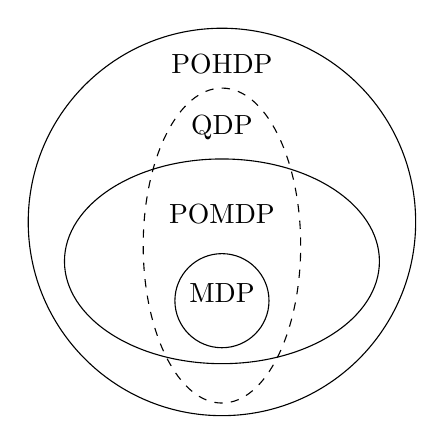
\begin{tikzpicture}
    \draw (0,0) circle (70pt) ;
    \node at (0,2) { POHDP };
    \draw (0,-0.5) circle [x radius = 2cm, y radius = 1.3cm]; % (40pt) ;
    \node at (0,0.1) { POMDP };
    \draw (0,-1) circle (17pt) ;
    \node at (0,-0.9) { MDP };
    \draw[dashed] (0, -0.3) circle [x radius=1cm, y radius=2cm];
    \node at (0,1.2) { QDP };
  \end{tikzpicture}
  \caption{Classes of finite decision processes considered in \ncite{MH18},
  under \cref{sett:HDP_MH}.}
  \label{fig:DPMH}
\end{figure}

Recall that QDP is a partially observable HDP under state-uniformity
(\cref{asm:stateUniformity}).

One point remains unclear after reading \ncite{MH18}:
Why is $q^*$ and $Q^*$ well defined as the solution to their
functional equations (\cref{eq:MH_Q_def} and \cref{eq:MH_q_def})
and how are they related to the optimal value function
$V^*(s) = \sup_{\pi \in R\Pi} \E_s^\pi
\sum_{i=1}^\infty \gamma^{i-1} r_i $
(see \cref{defn:optimalValue})
of a general HDP?
A sensible thing to ask would be that
$Q^*(h, a) = r(h, a) + \gamma \E_{P(\cdot \mid h a)} V^*$.
However we will not go further into these details.

\section{Results for continuous settings}

\subsection{Linear function approximation}

This section is based on \mcite{MR07}.

\begin{sett}[Melo, Rebeiro]
  \leavevmode
  \begin{enumerate}
    \item An MDP $(\cl{S}, \cl{A}, P, R, \gamma)$ (see \cref{sett:MDP}).
    \item Discounted, i.e. (D) holds with $\gamma \in [0,1)$.
    \item $\cl{S} \subseteq \R^w$ is compact.
    \item $\cl{A}$ is finite.
    \item $r_i$ is upper semicontinuous \label{item:MRlast}.
  \end{enumerate}
  \label{sett:MR}
\end{sett}

\begin{rem}
  \Cref{item:MRlast} was actually not part of the assumptions in
  \ncite{MR07}.
  We include it here in order to ensure the existence of an
  optimal policy and thus measurability of $V^*$.
\end{rem}

Let $\left\{ \xi_1, \dots, \xi_M \right\}$ be a finite set of linearly
independent, measurable and bounded action value functions,
$\xi_i : \cl{S} \times \cl{A} \to \R,\; \forall i \in [M]$.
Denote $\cl{Q} \defeq \Span\left\{ \xi_i \mid i \in [M] \right\}$
and for $\theta \in \R^M$
\[ Q_\theta(s, a) = \sum_{i=1}^M \theta_i \xi_i(s, a) = \xi^T \theta \]
Note that $\cl{Q} \subseteq \cl{L}_2(\cl{S}\times\cl{A})$ since any
$Q_\theta$ is bounded and $\cl{S}$ is compact (so closed and bounded).
We would now like to find the best approximation
$q^* \in \cl{Q}$ to $Q^*$ within the span.
If we measure distance by the $\cl{L}_2$-norm this is
simply $\rho_\cl{Q} Q^*$ where $\rho_\cl{Q}$ is the orthogonal projection on
$\cl{Q}$. Denote by $\theta^*$ the coordinates of this projection, i.e.
$\cl{Q}_{\theta^*} = \rho_\cl{Q} Q^*$.

The gradient of $Q_\theta$ over $\theta$ is
\[ \nabla_\theta Q_\theta(s, a) = \xi(s, a) \]
This gives the idea for a temporal difference with approximation from
$\cl{Q}$ using the update step
\[ \theta_{k+1} = \theta_k + \alpha_k \xi(s_k, a_k)
  \left( r_k + \gamma \max_{b \in \cl{A}} Q_{\theta_k}(s_{k+1}, b)
- Q_{\theta_k}(s_k, a_k) \right) \]

\begin{figure}[H]
\begin{algorithm}[H] %\label{algocf:fq} % this labels line, could not fix
  \caption{Q-learning with linear approximation}
  \KwIn{MDP $(\cl{S}, \cl{A}, P, R, \gamma)$,
    policy $\pi$,
    number of iterations $K$,
    learning rates $(\alpha_1, \dots, \alpha_K)$,
    initial $\theta_1 \in \R^M$
  }

  \For{$k = 1,2,\dots,K$}{
    Sample $a_k \sim \pi(\cdot \mid s_k)$,
    $s_{k+1} \sim P(\cdot \mid s_k, a_k)$,
    $r_k \sim R(\cdot \mid s_k, a_k)$.

    Update action-value parameter:
    \[ \theta_{k+1} = \theta_k + \alpha_k \xi(s_k, a_k)
      \left( r_k + \gamma \max_{b \in \cl{A}} Q_{\theta_k}(s_{k+1}, b)
    - Q_{\theta_k}(s_k, a_k) \right) \]
  }
  Define $\wt{\pi}_K$ as the greedy policy w.r.t.
  $\wt{Q}_K \defeq Q_{\theta_{K+1}}$.

  \KwOut{An estimator $\wt{Q}_K$ of $Q^*$ and policy $\wt{\pi}_K$}
  \label{alg:QLlinear}
\end{algorithm}
\end{figure}

In order to understand the results of the analysis of \cref{alg:QLlinear}
found in \ncite{MR07},
we need to define some concepts from ergodic theory.

Let $\kappa : \cl{X} \leadsto \cl{X}$ be a transition kernel.
Let $\fk{P} = \kappa^\infty : \cl{X} \leadsto \cl{X}^\infty$.
And denote by
$\fk{P}_x = \fk{P}\delta_x \in \cl{P}(\cl{X}^\infty)$
the probability measure for the process starting at $x \in \cl{X}$.
Let $\rho_i : \cl{X}^\infty \to \cl{X}$ be projection on the
$i$th space.
Define for any $A \in \Sigma_{\cl{X}}$ the function
$\tau_A : \cl{X}^\infty \to \ol{\N} = \inf\{ i \in \N \mid \rho_i \in A \}$.
Intuitively this function records the earliest time where the process
enter the set $A \subseteq \cl{X}$.
Define the function
$\eta_A : \cl{X}^\infty \to \ol{\N} = \sum_{i \in \N} 1_A \circ \rho_i$.
This function records the total number of times in which the process is
inside the set $A$.
Let $\varphi \in \cl{P}(\cl{X})$ be a probability measure on $\cl{X}$.

\begin{defn}[Invariant measure]
  A countably additive measure $\mu \in \cl{P}(\cl{X})$ is said
  to be \defemph{invariant} w.r.t $\kappa$ if $\kappa \circ \mu = \mu$.
\end{defn}

\begin{defn}[Positivity]
  \leavevmode

  $\fk{P}$ is called \defemph{positive} if it admits an $\kappa$-invariant
  probability measure $\mu$.
\end{defn}

\begin{defn}[Irreducibility]
  $\fk{P}$ is called $\varphi$-irreducible
  $\fk{P}_x(\tau_A < \infty) > 0$
  for all $A \in \Sigma_\cl{X}$
  with $\varphi(A) > 0$
  and all $x \in \cl{X}$.
\end{defn}

\begin{defn}[Harris recurrency]
  $\fk{P}$ is called $\varphi$-Harris recurrent if
  it it $\varphi$-irreducible and
  $\fk{P}_x(\eta_A = \infty) = 1$ for all $A \in \Sigma_\cl{X}$ with
  $\varphi(A) > 0$ and all $x \in \cl{X}$.
\end{defn}

\begin{defn}[Geometric ergodicity]
  A Markov process $\fk{P}$ is called \defemph{geometrically ergodic} if
  it is positive with invariant measure $\mu$, $\varphi$-Harris recurrent
  for some $\varphi \in \cl{P}(\cl{X})$ and $\exists t>1$ such that
  \[ \sum_{i=1}^\infty t^i \norm{P^n_x - \mu}_{TV} < \infty,
  \quad \forall x \in \cl{X} \]
\end{defn}

Since the $P,R$ of our MDP is reward independent we can view the
MDP as a stationary process $\fk{P}$ on $\cl{S}$
generated by kernel $P\pi$ for a policy $\pi \in S\Pi$.

\begin{thm}[Melo, Ribeiro]
  Let $(\cl{S}, \cl{A}, P, R, \gamma)$ be an MDP as of \cref{sett:MR}.
  Let $\pi \in S\Pi$ be a stationary process
  and $\fk{P}$ the process kernel derived by $P\pi$.
  Assume that $\fk{P}$ is geometrically ergodic with invariant
  measure $\mu$ and that
  $\pi(a \mid s) > 0$ for all $a \in \cl{A}$ and $\mu$-almost all
  $s \in \cl{S}$.
  Assume that $\sum_{i=1}^M \abs{\xi_i} \leq 1$.
  Then if \cref{alg:QLlinear} is run with learning rates from a sequence
  $\{ \alpha_k \}_{k \in \N}$ satisfying $\alpha_k \in [0,1]$ and
  \[ \sum_{k = 1}^\infty \alpha_k = \infty, \qquad
  \sum_{k = 1}^\infty \alpha_k^2 < \infty \]
  we have that
  \[ \theta_k \to \theta^* \]
  with probability 1, and $Q_{\theta^*}$ satisfies
  \[ Q_{\theta^*} = \rho_\cl{Q} T Q_{\theta^*} \]
  Furthermore the orthogonal projection is expressible as
  \[ \rho_\cl{Q} Q = \xi^T
    \frac{\E_{\pi\mu}\left( \xi Q \right)}{\E_{\pi\mu} (\xi \xi^T)}
  \]
  (recall the definition of the kernel-derived measure $\pi \mu(S \times A)
  = \int_S \pi(A \mid s) \difd \mu(s)$).
  \label{thm:MeloRibeiro}
\end{thm}

This gives us our first sort of convergence garantee for Q-learning in
continuous state space setting.
However there is still room for improvement since \cref{thm:MeloRibeiro}
does not tell us:
\begin{enumerate}
  \item How fast is the convergence?
  \item How far is $Q_{\theta^*}$ from $Q^*$?
    Though this is obviously best handled seperately for each $\cl{Q}$.
  \item How far is $Q_{\wt{\pi}_K}$ from $Q^*$?
\end{enumerate}
In a quite similar setting these questions are answered for the
fitted Q-iteration algorithm in the next section (\cref{thm:main}).

